\documentclass[border=10pt]{standalone}
\usepackage{tikz}
\usetikzlibrary{automata, positioning, arrows.meta}

\begin{document}
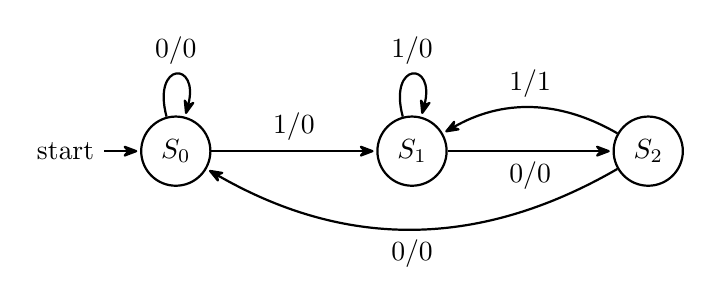
\begin{tikzpicture}[shorten >=1pt, node distance=3cm, on grid, auto, >={Stealth[round]}, thick]
    % Nodes
    \node[state, initial] (s0) {$S_0$};
    \node[state] (s1) [right=of s0] {$S_1$};
    \node[state] (s2) [right=of s1] {$S_2$};
    
    % Labels for state meanings can be added as label nodes if needed, or kept simple.
    % The user diagram had descriptions: S0 (Reset), S1 (Got '1'), S2 (Got '10')

    % Transitions (Mealy: Input/Output)
    \path[->]
        (s0) edge [loop above] node {0/0} (s0)
             edge node {1/0} (s1)
        (s1) edge [loop above] node {1/0} (s1)
             edge [swap] node {0/0} (s2)
        (s2) edge [bend left] node {0/0} (s0)
             edge [swap][bend right] node {1/1} (s1);
\end{tikzpicture}
\end{document}
